\documentclass[a4paper]{hitec}
\settextfraction{0.95}      % reduce left margin

\usepackage{styles/main}
\usepackage{styles/custom}
\usepackage{pdfpages,commath}

\labtitle{Spannungsstabilisierung}

\author{Rene Hampölz, Gruppe 6}
\company{HTBLA Weiz, 5BHET}
\date{17. Oktober 2022}

\begin{document}

\maketitle

\tableofcontents

\clearpage

\section{Einführung}

Es soll eine einfache Spannungsstabilisierung/steuerung mit einer Kollektorschaltung dimensioniert und aufgebaut werden.
Des Weiteren soll als Vergleich eine Spannungsstabilisierung/regelung mit einem Operationsverstärker dimensioniert und aufgebaut werden.
Mit Simulationen sollen die Funktionsweisen der Schaltungen überprüft werden.

\begin{sagesilent}
    I_a_max = 0.05
    I_ZD = 0.001

    U_ZD = 5.1
    U_ZD_max = 5.4
    U_BE = 0.66
    U_O_OPV = 13.8
\end{sagesilent}

Allgemeine Angaben: $I_{a_{max}} = \SIvar{I_a_max}{\ampere}$, $I_{ZD} = \SIvar{I_ZD}{\ampere}$

Datenblatt: $U_{ZD} = \SIvar{U_ZD}{\volt}$, $U_{ZD} = \SIvar{U_ZD}{\volt}$, $U_{ZD_{max}} = \SIvar{U_ZD_max}{\volt}$, $U_{BE} = \SIvar{U_BE}{\volt}$, $U_{O_{OPV}} = \SIvar{U_O_OPV}{\volt}$

\vspace{1cm}

\section{Spannungsstabilisierung mit Kollektorschaltung}

\subsection{Einführung}

Die Basis eines NPN-Transistors ist an einem Spannungsteiler durch $R_{V}$ und der Z-Diode $ZD$ angeschlossen. Die Spannung an der Z-Diode $U_{ZD}$ bleibt nahezu konstant.
Somit wird die Spannungsdifferenz $U_{BE}$ zwischen Basis und Emitter des Transistors kleiner, wenn die Ausgangsspannung $U_{a}$ \textit{(welche am Emitter anliegt)} steigt.
Dadurch verringert sich der Basisstrom $I_{B}$ sowie auch der Kollektor- und Emitterstrom bzw. der Ausgangsstrom $I_{a}$, aufgrund der Stromverstärkung des Transistors.
Dies führt dazu, dass die Ausgangsspannung bei Laständerungen konstant bleibt.   

\begin{sagesilent}
    U_e0 = 10
\end{sagesilent}

Schaltungsspezifische Angaben: $U_{e0} = \SIvar{U_e0}{\volt}$

\subsection{Schaltung}

\begin{figure}[H]
    \centering
    \begin{circuitikz}
        \coordinate (in+) at (0,0);
        \coordinate (in-) at (0,-5);

        \draw
        (in+) to[short,o-] ++(2,0) coordinate (aux1)
        to[R=$R_{V}$,*-*] ++(0,-2) coordinate (aux2)
        to[zD=$ZD$,name=ZD,i>^,invert,*-*] (aux2 |- in-)

        (aux2) ++(2,0) node[npn] (T) {$T$}
        (T.E) coordinate (out+)

        (aux2) to[short,name=I_B,i] (T.B)
        (aux1) -- (aux1 -| T.C) -- (T.C)

        (out+) to[R=$R_{L}$,name=R_L,i>^,o-o] (out+ |- in-) coordinate (out-)

        (in-) to[short,o-] (out-)

        (in+) to[open,name=inV,v] (in-)
        ($(out+) + (1,0)$) to[open,name=outV,v^] ($(out-) + (1,0)$)
        ;

        \voltage{inV}{$U_{e0}$}
        \current{ZD}{$I_{ZD}$}
        \current{I_B}{$I_{B}$}
        \current{R_L}{$I_{a}$}
        \voltage{outV}{$U_{a}$}
    \end{circuitikz}
\end{figure}

\subsection{Berechnungen}

\subsubsection{Vorwiderstand $R_V$}

Um den von der Z-Diode benötigten Strom $I_{ZD}$ zu liefern und um den Arbeitspunkt einzustellen, wird der Vorwiderstand $R_{V}$ benötigt.
Die Eingangsspannung $U_{e0}$ fällt somit an der Z-Diode $ZD$ sowie am Vorwiderstand $R_{V}$ ab:

\begin{sagesilent}
    U_R_V = U_e0 - U_ZD
\end{sagesilent}

\begin{align*}
    U_{R_{V}} &= U_{e0} - U_{ZD} \\
    U_{R_{V}} &= \var{U_e0} - \var{U_ZD} \\
    U_{R_{V}} &= \SIvar{U_R_V}{\volt}
\end{align*}

\pagebreak

Der Strom, welcher durch den Vorwiderstand $R_{V}$ fließt, setzt sich aus dem Strom $I_{ZD}$ der Z-Diode und dem Basis-Strom $I_{B}$ des Transistors zusammen.
Der Basis-Strom $I_{ZD}$ ist jedoch meist so klein, dass dieser vernachlässigt werden kann.

Nach dem Ohmschen Gesetz ergibt sich somit der Vorwiderstand $R_{V}$:

\begin{sagesilent}
    R_V = U_R_V / I_ZD # + I_B (= <<) 
\end{sagesilent}

\begin{equation*}
    R_{V} = \frac{U_{R_{V}}}{I_{ZD} + I_{B}} \tag*{$I_{B} = \quad \ll$ \quad \textit{(vernachlässigbar)}}
\end{equation*}

\begin{align*}
    R_{V} &= \frac{U_{R_{V}}}{I_{ZD}} \\
    R_{V} &= \frac{\var{U_R_V}}{\var{I_ZD}} \\
    R_{V} &= \SIvar{R_V}{\ohm}
\end{align*}

\subsubsection{Minimaler Lastwiderstand $R_{L_{min}}$}

Die Zener-Spannung $U_{ZD}$ \textit{(bzw. $U_{ZD_{max}}$, da der minimale Lastwiderstand gesucht ist)} teilt sich in die Basis-Emitter-Spannung $U_{BE}$ des Transistors und in die Ausgangsspannung $U_{a}$ \textit{(bzw. $U_{a_{max}}$)} auf.
Daraus ergibt sich für die maximale Lastspannung $U_{a_{max}}$: 

\begin{sagesilent}
    U_a_max = U_ZD_max - U_BE
\end{sagesilent}

\begin{align*}
    U_{a_{max}} &= U_{ZD_{max}} - U_{BE} \\
    U_{a_{max}} &= \var{U_ZD_max} - \var{U_BE} \\
    U_{a_{max}} &= \SIvar{U_a_max}{\volt}
\end{align*}

Nach dem Ohmschen Gesetz ergibt sich schließlich der minimale Lastwiderstand $R_{L_{min}}$:

\begin{sagesilent}
    R_L_min = U_a_max / I_a_max
\end{sagesilent}

\begin{align*}
    R_{L_{min}} = \frac{U_{a_{max}}}{I_{a_{max}}} \\
    R_{L_{min}} = \frac{\var{U_a_max}}{\var{I_a_max}} \\
    R_{L_{min}} = \SIvar{R_L_min}{\ohm}
\end{align*}

\subsection{Simulation}

\begin{sagesilent}
    simulation1_data = LTSpice.plot_data("src/simulations/export/01 Spannungs-Stabilisierung_Kollektor.txt")
    simulation1_data_Vout = simulation1_data["V(out)"]

    simulation1_plot = list_plot(
        simulation1_data_Vout,
        axes_labels=['$R_L$ in $\Omega$', '$U_a$ in V'],
        figsize=[5.5,2],
        plotjoined=True,
        frame=True
    )
\end{sagesilent}

\begin{figure}[H]
    \centering
    \sageplot{simulation1_plot}
    \caption{Ausgangskennlinie \textbf{$U_{a} = f(R_L)$} der Simulation}
    \label{fig:simulation1}
\end{figure}

\vspace{-1em}

Die Simulation konnte nicht mit der gleichen Z-Diode wie bei der Messung durchgeführt werden.
Daher weicht der Wertebereich in der Ausgangskennlinie der Simulation \textit{(Abb. \ref{fig:simulation1})} etwas von dem der Messung \textit{(Abb. \ref{fig:measure1})} ab.

\subsection{Auswertung}

\begin{sagesilent}
    measures = Measures(
        [
            '$R_L$ in $\Omega$',
            '$U_a$ in V', 
            '$I_a$ in mA'
        ], [
            ['100', '3.96', '38.2'],
            ['120', '3.96', '32.0'],
            ['130', '3.93', '29.5'],
            ['140', '3.94', '27.4'],
            ['150', '3.95', '25.7'],
            ['160', '3.94', '24.1'],
            ['170', '3.92', '22.6'],
            ['200', '3.91', '19.2'],
            ['250', '3.95', '15.6'],
            ['300', '3.98', '13.2'],
            ['400', '4.05', '10.0'],
            ['500', '4.10', '8.2'],
            ['600', '4.17', '6.95'],
            ['700', '4.22', '6.00'],
            ['800', '4.23', '5.30'],
            ['1000', '4.29', '4.30'],
            ['2000', '4.30', '2.16'],
        ], ndigits=[0, 2, 1])

    index_RL = 0
    index_Ua = 1
    index_Ia = 2
\end{sagesilent}

\subsubsection{Messwerte}

\begin{center}
    \renewcommand{\arraystretch}{1.2}
    \var{measures.table}
\end{center}

\subsubsection{Grafische Darstellung}

\begin{sagesilent}
    f = list_plot(
        measures.plot_data(index_RL, index_Ua),
        axes_labels=['$R_L$ in $\Omega$', '$U_a$ in V'],
        figsize=[5.5,2],
        color='purple'
    )

    f += line(
        measures.g1d_smooth(index_RL, index_Ua, sigma=0.75, connect=True),
        linestyle="--",
        color='blue'
    )

    f += line(
        [(100, 4), (100, 3.9)],
        linestyle=":",
        color="red"
    )

    f += line(
        [(200, 4), (200, 3.9)],
        linestyle=":",
        color="red"
    )
\end{sagesilent}

\begin{figure}[H]
    \centering
    \sageplot{f}
    \caption{Ausgangskennlinie \textbf{$U_{a} = f(R_L)$} mit gemessene Werte}
    \label{fig:measure1}
\end{figure}

Die Schwankungen der Ausgangsspannung $U_{a}$ im Bereich von $\qty{100}{\ohm} \to \qty{200}{\ohm}$ in der Ausgangskennlinie mit gemessenen Werte \textit{(Abb. \ref{fig:measure1})} sind auf mögliche Störgrößen, wie Änderungen der Eingangsspannung oder Erwärmung der Bauteile, zurückzuführen.

\subsubsection{Bemerkung}

Die Schaltung liefert ab dem ermittelten minimalen Lastwiederstand $R_{L_{min}}$ eine annähernd konstante und stabile Ausgangsspannung $U_{a}$ mit Abweichungen von wenigen Millivolt.
Bei größeren Lastwiederständen verhält sich die Ausgangsspannung etwas stabiler.
Da die Schaltung jedoch keine Rückkopplung besitzt, ist sie sehr anfällig für Störgrößen.

\subsection{Verwendete Geräte}

\medskip

\begin{devicelist}
    \devicecat{Widerstands-Dekade}{2}{%
        \device{ET-MTL1-RD23}{R_{V}}
        \device{ET-MTL1-RD29}{R_{L}}
    }
    \devicecat{Multimeter}{2}{%
        \device{ET-MTL1-DM20}{I_{a}}
        \device{ET-MTL1-DM22}{U_{a}}
    }
    \devicecat{Z-Diode}{1}{%
        \device{BZD23-C5V1}{ZD}
    }
    \devicecat{Transistor}{1}{%
        \device{BC546C}{T}
    }
\end{devicelist}

\clearpage

\section{Spannungsstabilisierung mit Operationsverstärker}

\subsection{Einführung}

Der Operationsverstärker führt einen Soll-Istwert Vergleich durch. Dabei wird eine Referenzspannung mit der Spannung der Rückkopplung verglichen.
Eine Differenz der beiden Spannungen führt zu einer Ausgangsspannung.  

Für die Referenzspannungsquelle wird eine einfache Z-Dioden Stabilisierung mit dem Widerstand $R_{V}$ und der Z-Diode $ZD$ verwendet.

Die Referenzspannungsquelle wird an den nichtinvertierenden Eingang des OPVs angeschlossen.
Am invertierenden Eingang wird \textit(für die Rückkopplung) über die Widerstände $R_{1}$ und $R_{2}$ der Sollwert der Ausgangsgröße beeinflusst.
Der Ausgang des OPVs steuert schließlich einen NPN-Transistor, welcher somit auch den Ausgangsstrom $I_{a}$ steuert, um die Ausgangsspannung bei Laständerungen konstant zu halten.   

Die Ausgangsspannung $U_{a}$ kann auf einen beliebigen Wert zwischen der Zener-Spannung $U_{ZD}$ und (fast) der Eingangsspannung $U_{e0}$ eingestellt werden.

\begin{sagesilent}
    U_e0 = 15
    U_a = 7
\end{sagesilent}

Schaltungsspezifische Angaben: $U_{e0} = \SIvar{U_e0}{\volt}$, $U_{a} = \SIvar{U_a}{\volt}$

\subsection{Schaltung}

\begin{figure}[H]
    \centering
    \begin{circuitikz}
        \coordinate (in+) at (0,0);
        \coordinate (in-) at (0,-6);

        \draw
        (in+) to[short,o-] ++(2,0) coordinate(aux1)
        to[R=$R_{V}$,*-*] ++(0,-2) coordinate(aux2)
        to[zD=$ZD$,name=ZD,i>^,invert,*-*] (aux2 |- in-)

        (aux2) -- ++(2,0) node[op amp,noinv input up,anchor=+](OPV){OPV}
        (OPV.-) -- ++(0,-1) coordinate(opv-aux1)
        
        (aux1) -- ++(4,0) node[npn,rotate=90,anchor=C](T){\rotatebox{-90}{$T$}}
        (T.B) -- (T.B |- OPV.out) -- (OPV.out)
        (T.E) -- ++(2,0) coordinate(aux3) to[short,name=outI,i] ++(2,0) coordinate(out+)

        (aux3) to[R=$R_{1}$,*-*] (aux3 |- opv-aux1) coordinate(aux4) -- (opv-aux1)
        (aux4) to[R=$R_{2}$,*-*] (aux4 |- in-)

        (out+) to[R=$R_{L}$,o-o] (out+ |- in-) coordinate(out-)

        (in-) to[short,o-] (out-)

        (in+) to[open,name=inV,v] (in-)
        ($(out+) + (1,0)$) to[open,name=outV,v^] ($(out-) + (1,0)$)
        ;

        \voltage{inV}{$U_{e0}$}
        \current{ZD}{$I_{ZD}$}
        \current{outI}{$I_{a}$}
        \voltage{outV}{$U_{a}$}
    \end{circuitikz}
\end{figure}

\subsection{Berechnungen}

\subsubsection{Widerstand $R_{V}$ der Referenzspannungsquelle}

Um den von der Z-Diode benötigten Strom $I_{ZD}$ zu liefern, wird der Vorwiderstand $R_{V}$ benötigt.
Die Eingangsspannung $U_{e0}$ fällt somit an der Z-Diode $ZD$ sowie am Vorwiderstand $R_{V}$ ab:

\begin{sagesilent}
    U_R_V = U_e0 - U_ZD
\end{sagesilent}

\begin{align*}
    U_{R_{V}} &= U_{e0} - U_{ZD} \\
    U_{R_{V}} &= \var{U_e0} - \var{U_ZD} \\
    U_{R_{V}} &= \SIvar{U_R_V}{\volt}
\end{align*}

\pagebreak

Nach dem Ohmschen Gesetz ergibt sich somit der Vorwiderstand $R_{V}$:

\begin{sagesilent}
    R_V = U_R_V / I_ZD
\end{sagesilent}

\begin{align*}
    R_{V} &= \frac{U_{R_{V}}}{I_{ZD}} \\
    R_{V} &= \frac{\var{U_R_V}}{\var{I_ZD}} \\
    R_{V} &= \SIvar{R_V}{\ohm}
\end{align*}

\subsubsection{Widerstände $R_{1}$ und $R_{2}$ der Sollwerteinstellung}

Um den Sollwert der Ausgangsspannung $U_{a}$ zu beeinflussen, werden die beiden Widerstände $R_{1}$ und $R_{2}$ benötigt.
Ohne dieser Sollwerteinstellung würde am Ausgang die Referenzspannung anliegen. \\

Nach dem Kirchhoffschen Gesetz ergeben sich folgende Machenregeln und somit auch die Spannungsabfälle der Widerstände:

\begin{sagesilent}
    U_R_1_max = U_O_OPV - U_BE
    U_R_2_max = U_a - U_R_1_max
\end{sagesilent}

\begin{align*}
    U_{O_{OPV}} &= U_{BE} + U_{R_{1_{(max)}}} \\
    U_{R_{1_{(max)}}} &= U_{O_{OPV}} - U_{BE} \\
    U_{R_{1_{(max)}}} &= \var{U_O_OPV} - \var{U_BE} \\
    U_{R_{1_{(max)}}} &= \SIvar{U_R_1_max}{\volt}
\end{align*}

\begin{align*}
    U_{a} &= U_{R_{1_{(max)}}} + U_{R_{2_{(max)}}} \\
    U_{R_{2_{(max)}}} &= U_{a} - U_{R_{1_{(max)}}} \\
    U_{R_{2_{(max)}}} &= \var{U_a} - \var{U_R_1_max} \\
    U_{R_{2_{(max)}}} &= \SIvar{U_R_2_max}{\volt}
\end{align*}

\begin{sagesilent}
    I_R_12_max = 0.01
\end{sagesilent}

Mit diesen Werten kann schließlich das Widerstands-Verhältnis der beiden Widerstände ermittelt werden. Aufgrund der negativen Spannung $U_{R_{2_{(max)}}}$ kehrt sich das Verhältnis um:

\begin{sagesilent}
    R_12_multiplier = 100

    R_1 = floor(abs(U_R_2_max))*R_12_multiplier
    R_2 = floor(U_R_1_max)*R_12_multiplier
\end{sagesilent}

\begin{align*}
    \frac{R_{1}}{R_{2}} &\sim - \frac{U_{R_{1_{(max)}}}}{\abs{U_{R_{2_{(max)}}}}} \\
    \frac{R_{1}}{R_{2}} &\sim \frac{\abs{U_{R_{2_{(max)}}}}}{U_{R_{1_{(max)}}}} \\
    \frac{R_{1}}{R_{2}} &\sim \frac{\var{abs(U_R_2_max)}}{\var{U_R_1_max}} \\
    \frac{R_{1}}{R_{2}} &\sim \frac{\SIvar{R_1}{\ohm}}{\SIvar{R_2}{\ohm}}
\end{align*}

Die tatsächlichen Widerstandswerte wurden unter Berücksichtigung des erforderlichen Widerstandsverhältnis frei angenommen.\\

Für ein vorhersehbareres Schaltungsverhalten sollten die Widerstandswerte jedoch über einen gewählten maximal fließenden Strom berechnet werden.

\subsubsection{Minimaler Lastwiderstand $R_{L_{min}}$}

Der minimale Lastwiderstand $R_{L_{min}}$ wird schließlich durch das Ohmsche Gesetz mit der vorgesehenen konstanten Ausgangsspannung $U_{a}$ und mit dem maximal fließenden Ausgangsstrom $I_{a_{max}}$ berechnet:

\begin{sagesilent}
    R_L_min = U_a / I_a_max
\end{sagesilent}

\begin{align*}
    R_{L_{min}} &= \frac{U_{a}}{I_{a_{max}}} \\
    R_{L_{min}} &= \frac{\var{U_a}}{\var{I_a_max}} \\
    R_{L_{min}} &= \SIvar{R_L_min}{\ohm}
\end{align*}

\subsection{Simulation}

\begin{sagesilent}
    simulation2_data = LTSpice.plot_data("src/simulations/export/02 Spannungs-Stabilisierung_OPV.txt")
    simulation2_data_Vout = simulation2_data["V(out)"]

    simulation2_plot = list_plot(
        simulation2_data_Vout,
        axes_labels=['$R_L$ in $\Omega$', '$U_a$ in V'],
        figsize=[5.5,2],
        plotjoined=True,
        frame=True
    )
\end{sagesilent}

\begin{figure}[H]
    \centering
    \sageplot{simulation2_plot}
    \caption{Ausgangskennlinie \textbf{$U_{a} = f(R_L)$} der Simulation}
    \label{fig:simulation2}
\end{figure}

Die Simulation konnte nicht mit der gleichen Z-Diode wie bei der Messung durchgeführt werden.
Daher weicht der Wertebereich in der Ausgangskennlinie der Simulation \textit{(Abb. \ref{fig:simulation2})} etwas von dem der Messung \textit{(Abb. \ref{fig:measure2})} ab.

\subsection{Auswertung}

\subsubsection{Messwerte}

\begin{sagesilent}
    measures = Measures(
        [
            '$R_L$ in $\Omega$',
            '$U_a$ in V', 
            '$I_a$ in mA'
        ], [
            ['140', '6.8', '47'],
            ['160', '6.8', '41'],
            ['200', '6.8', '33'],
            ['250', '6.8', '27'],
            ['300', '6.8', '22'],
            ['400', '6.8', '17'],
            ['500', '6.8', '13'],
            ['1000', '6.8', '7'],
    ], ndigits=[0, 1, 0])

    index_RL = 0
    index_Ua = 1
    index_Ia = 2
\end{sagesilent}

\begin{center}
    \renewcommand{\arraystretch}{1.2}
    \var{measures.table}
\end{center}

\subsubsection{Grafische Darstellung}

\begin{sagesilent}
    f = list_plot(
        measures.plot_data(index_RL, index_Ua),
        axes_labels=['$R_L$ in $\Omega$', '$U_a$ in V'],
        figsize=[5.5,2],
        ticks=[100,0.4],
        color='purple'
    )

    f += line(
        measures.plot_data(index_RL, index_Ua),
        linestyle="--",
        color='blue'
    )
\end{sagesilent}

\begin{figure}[H]
    \centering
    \sageplot{f}
    \caption{Ausgangskennlinie \textbf{$U_{a} = f(R_L)$} mit gemessene Werte}
    \label{fig:measure2}
\end{figure}

\subsubsection{Bemerkung}

Die Schaltung liefert ab dem ermittelten minimalen Lastwiederstand $R_{L_{min}}$ eine komplett konstante und stabile Ausgangsspannung $U_{a}$ ohne erkennbare Abweichungen.

Da die Schaltung eine Rückkopplung besitzt, kann die Ausgangsspannung \textit{(im Gegensatz zur Spannungsstabilisierung mit Kollektorschaltung)} trotz möglicher Störgrößen stabil geregelt werden.

\subsection{Verwendete Geräte}

\begin{devicelist}
    \devicecat{Widerstands-Dekade}{2}{%
        \device{ET-MTL1-RD09}{R_V}
        \device{ET-MTL1-RD14}{R_1}
        \device{ET-MTL1-RD28}{R_2}
        \device{ET-MTL1-RG26}{R_L}
    }
    \devicecat{Multimeter}{2}{%
        \device{ET-MTL1-DM20}{I_a}
        \device{ET-MTL1-DM22}{U_a}
    }
    \devicecat{Z-Diode}{1}{%
        \device{BZD23-C5V1}{ZD}
    }
    \devicecat{Transistor}{1}{%
        \device{BC546C}{T}
    }
    \devicecat{Operationsverstärker}{1}{%
        \device{OP27}{\text{OPV}}
    }
\end{devicelist}

\clearpage

\IncludeHistoryTimeline

\clearpage

\invisiblesection{Datenblätter}
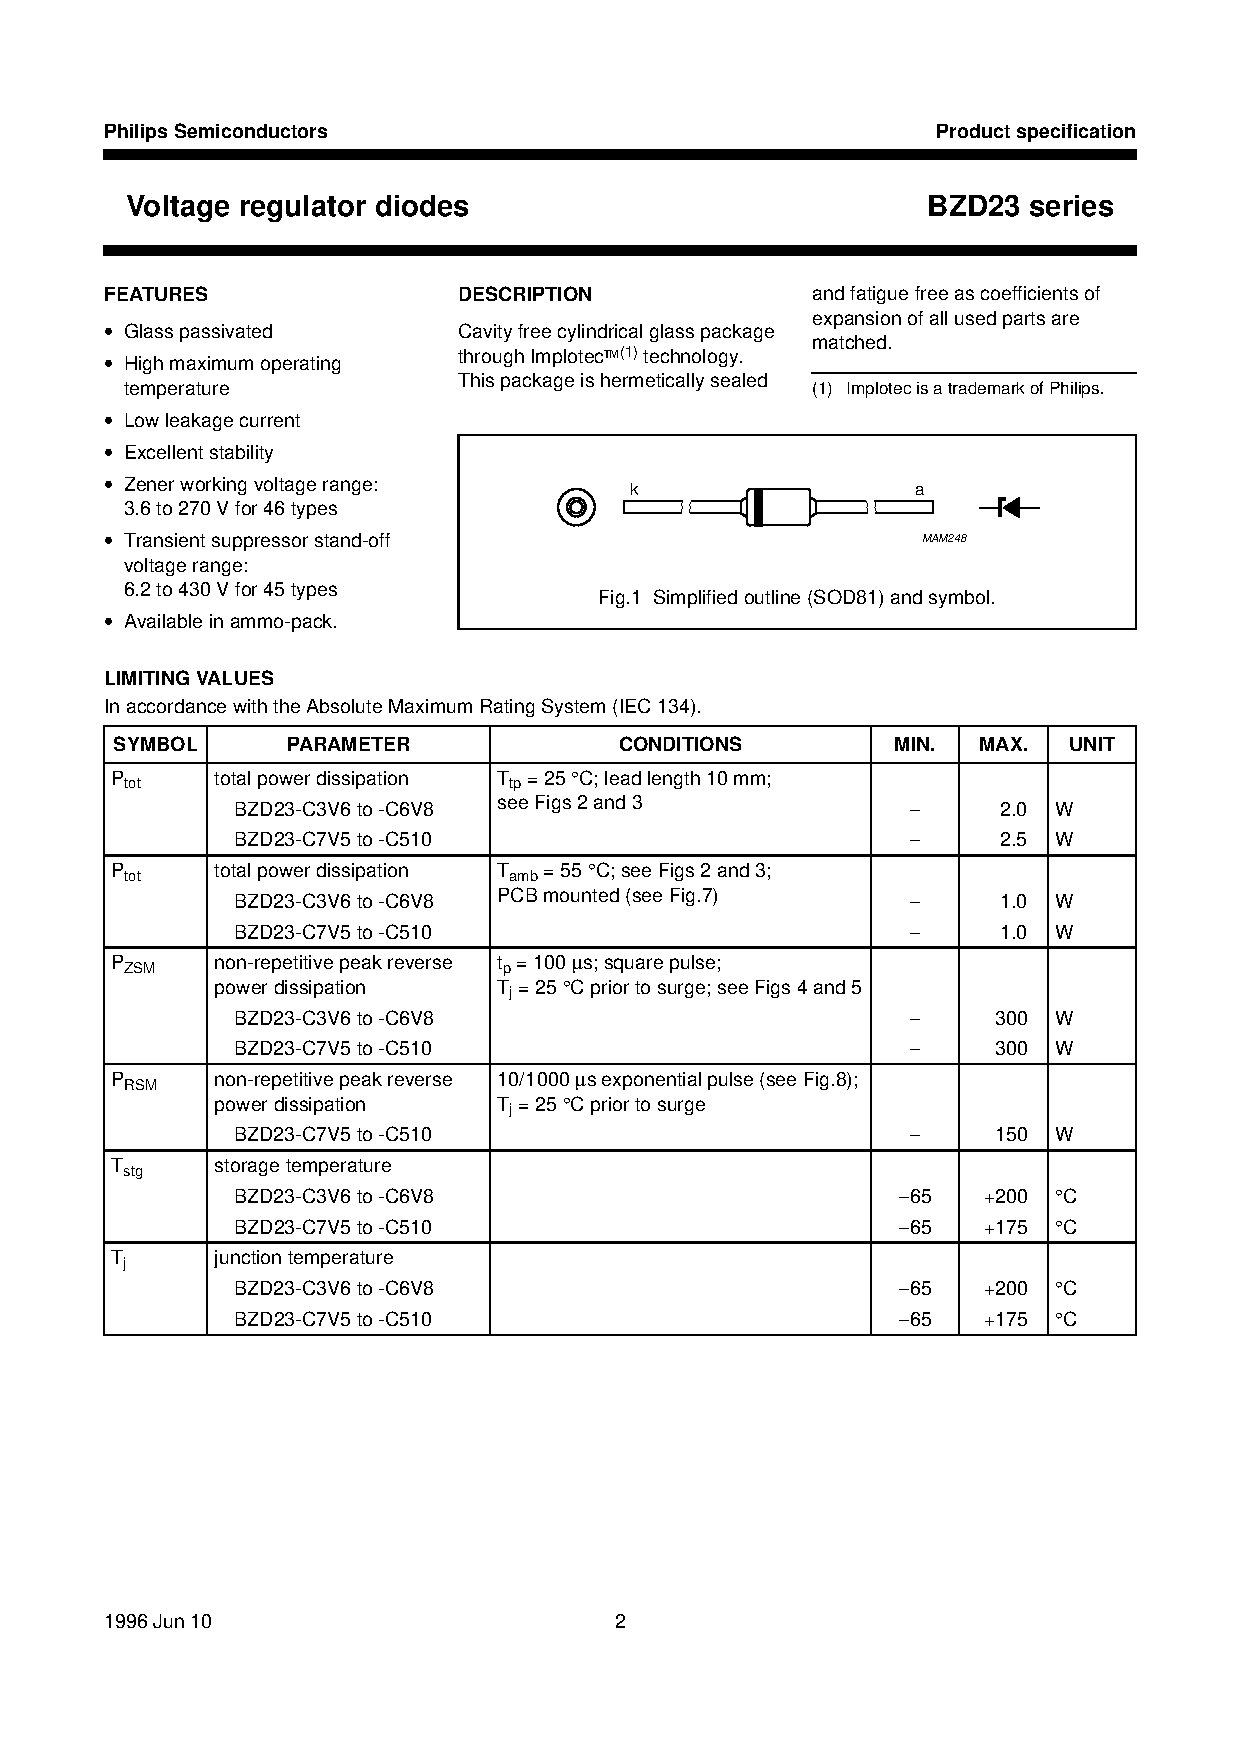
\includepdf[pages={1-}, addtotoc={1,subsection,2,BZD23-C5V1,datasheet:BZD23-C5V1}]{src/datasheets/BZD23-C5V1.pdf}
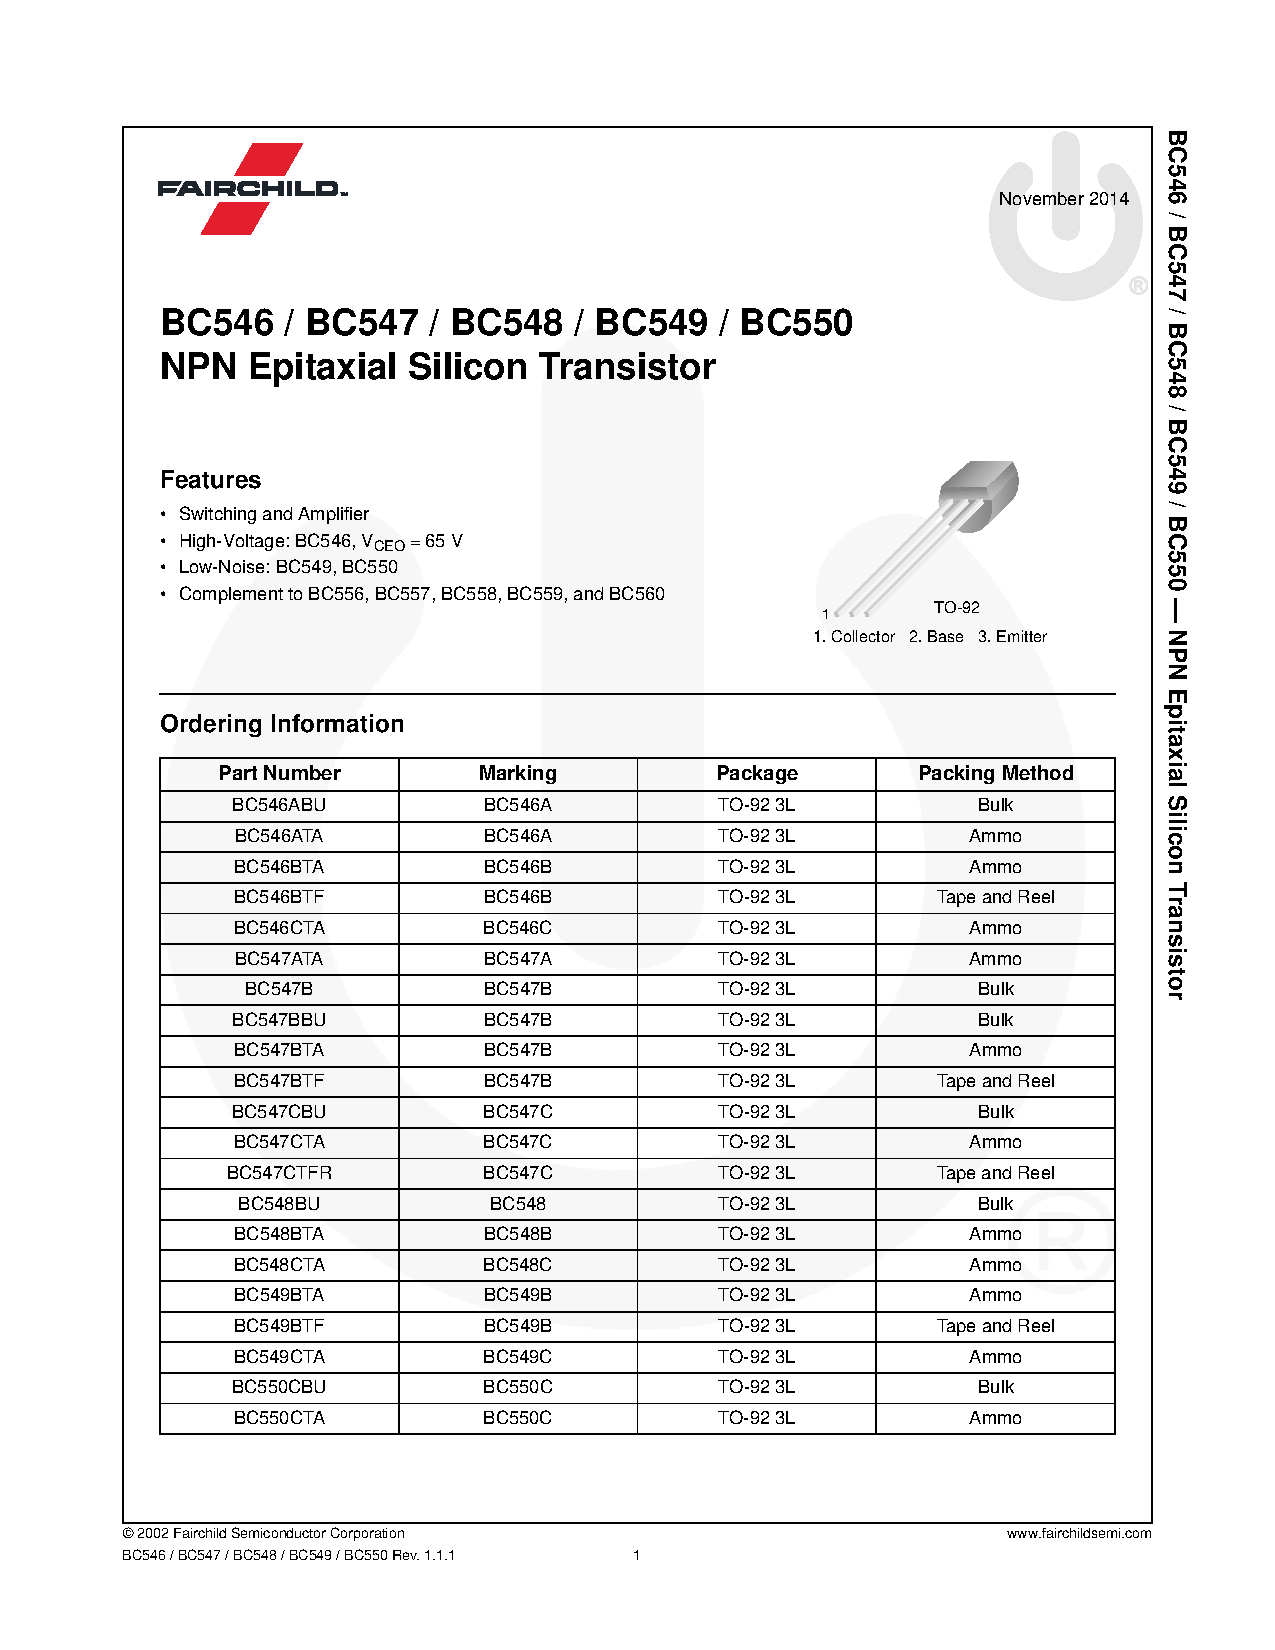
\includepdf[pages={1-}, addtotoc={1,subsection,2,BC546C,datasheet:BC546C}]{src/datasheets/BC546C.pdf}
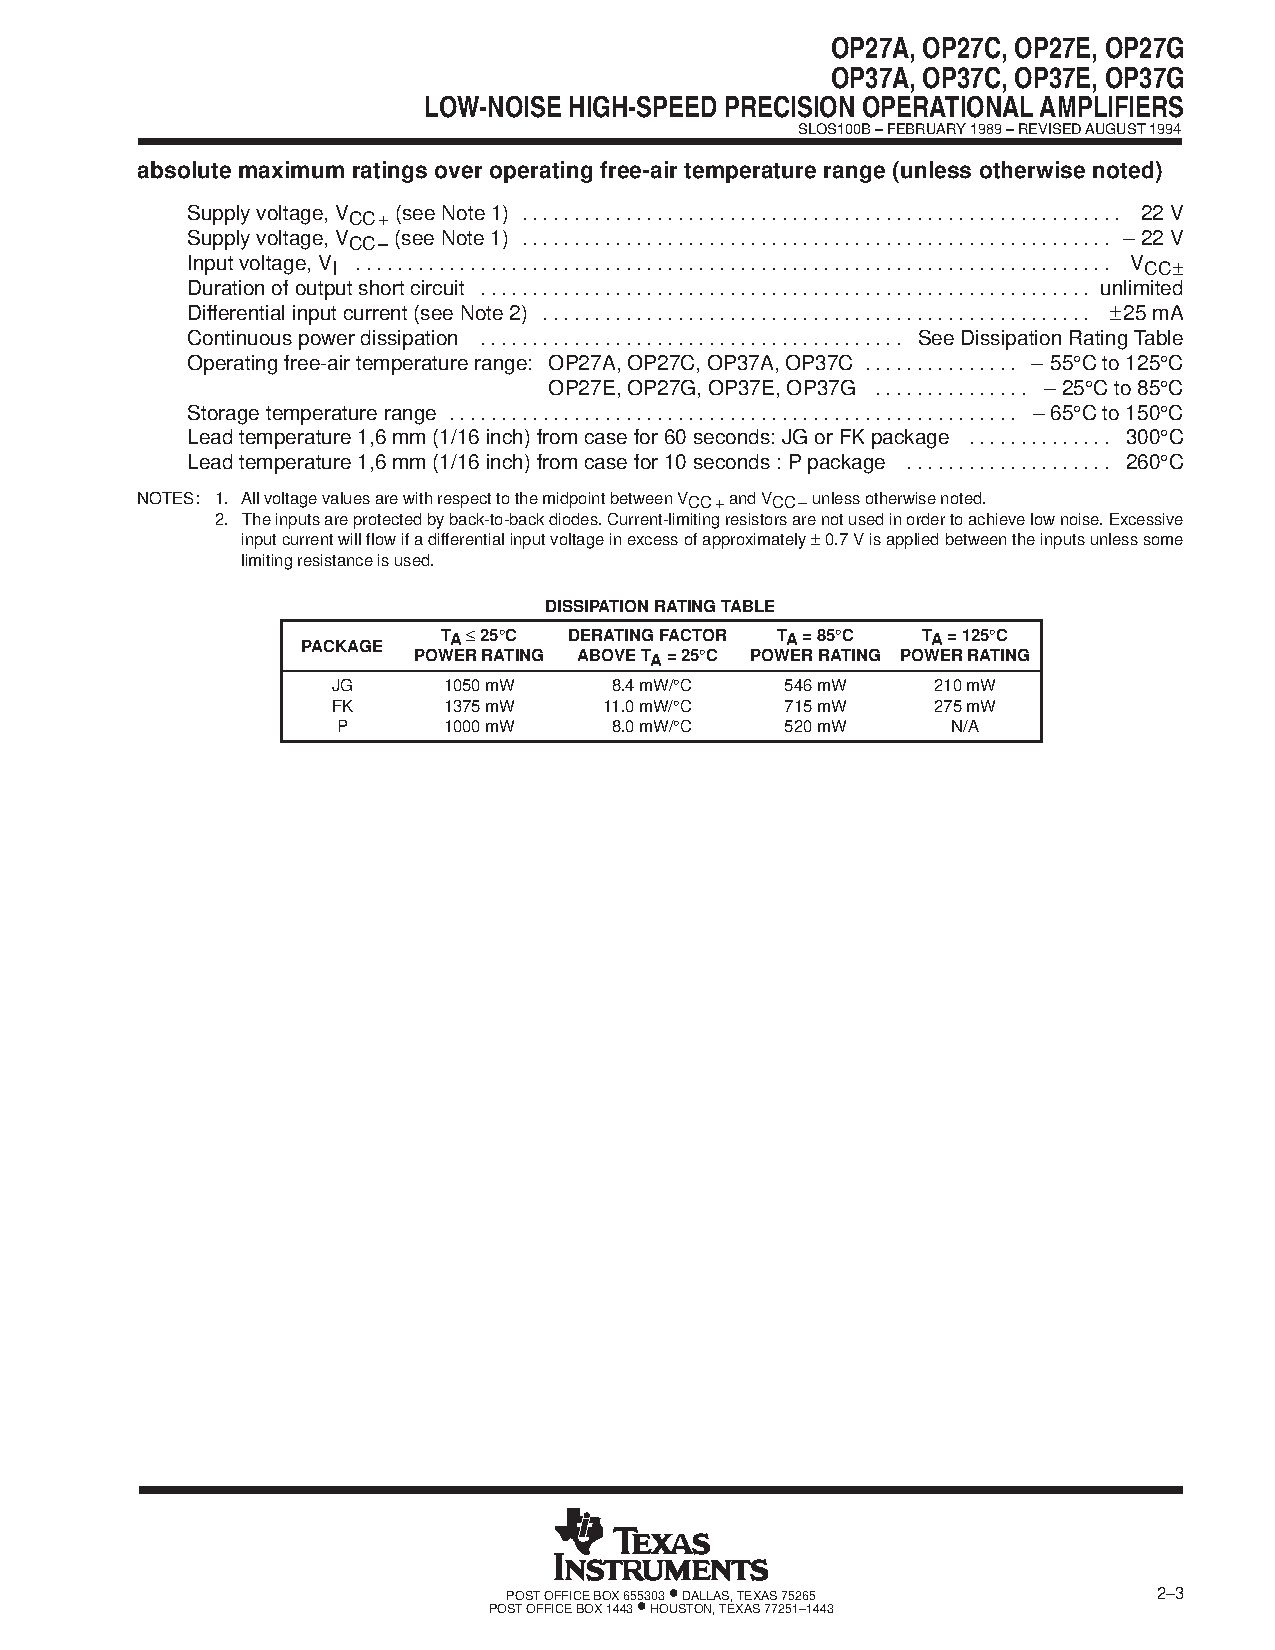
\includepdf[pages={1-}, addtotoc={1,subsection,2,OP27,datasheet:OP27}]{src/datasheets/OP27.pdf}

\end{document}